\subsection{تخمین پارامترهای کانال رول}
برای اصلاح پارامترهای رول چندین آزمایش انجام شد و با استفاده از داده‌های ثبت شده از وضعیت استند در کانال رول و جعبه‌ابزار
\lr{Parameter Estimator}،
پارامترهای کانال رول اصلاح شدند.
برای انجام آزمایش هر یک از موتورهای دو و چهار  با دور مختلف شروع به حرکت کردند و از خروجی سنسور داده برداری شد. سپس، مدل و داده‌های ثبت شده‌ی سنسور (وضعیت استند در کانال رول) به جعبه‌ابزار
\lr{Parameter Estimator}
داده شد. وضعیت کانال رول استند در شبیه‌سازی و واقعیت بعد از اصلاح پارامترهای کانال رول در شکل‌های
\ref{roll_ps1}, \ref{roll_ps2}, \ref{roll_ps3}, \ref{roll_ps4} و \ref{roll_ps5}
مقایسه شده است.
%
%\begin{figure}[H]
%	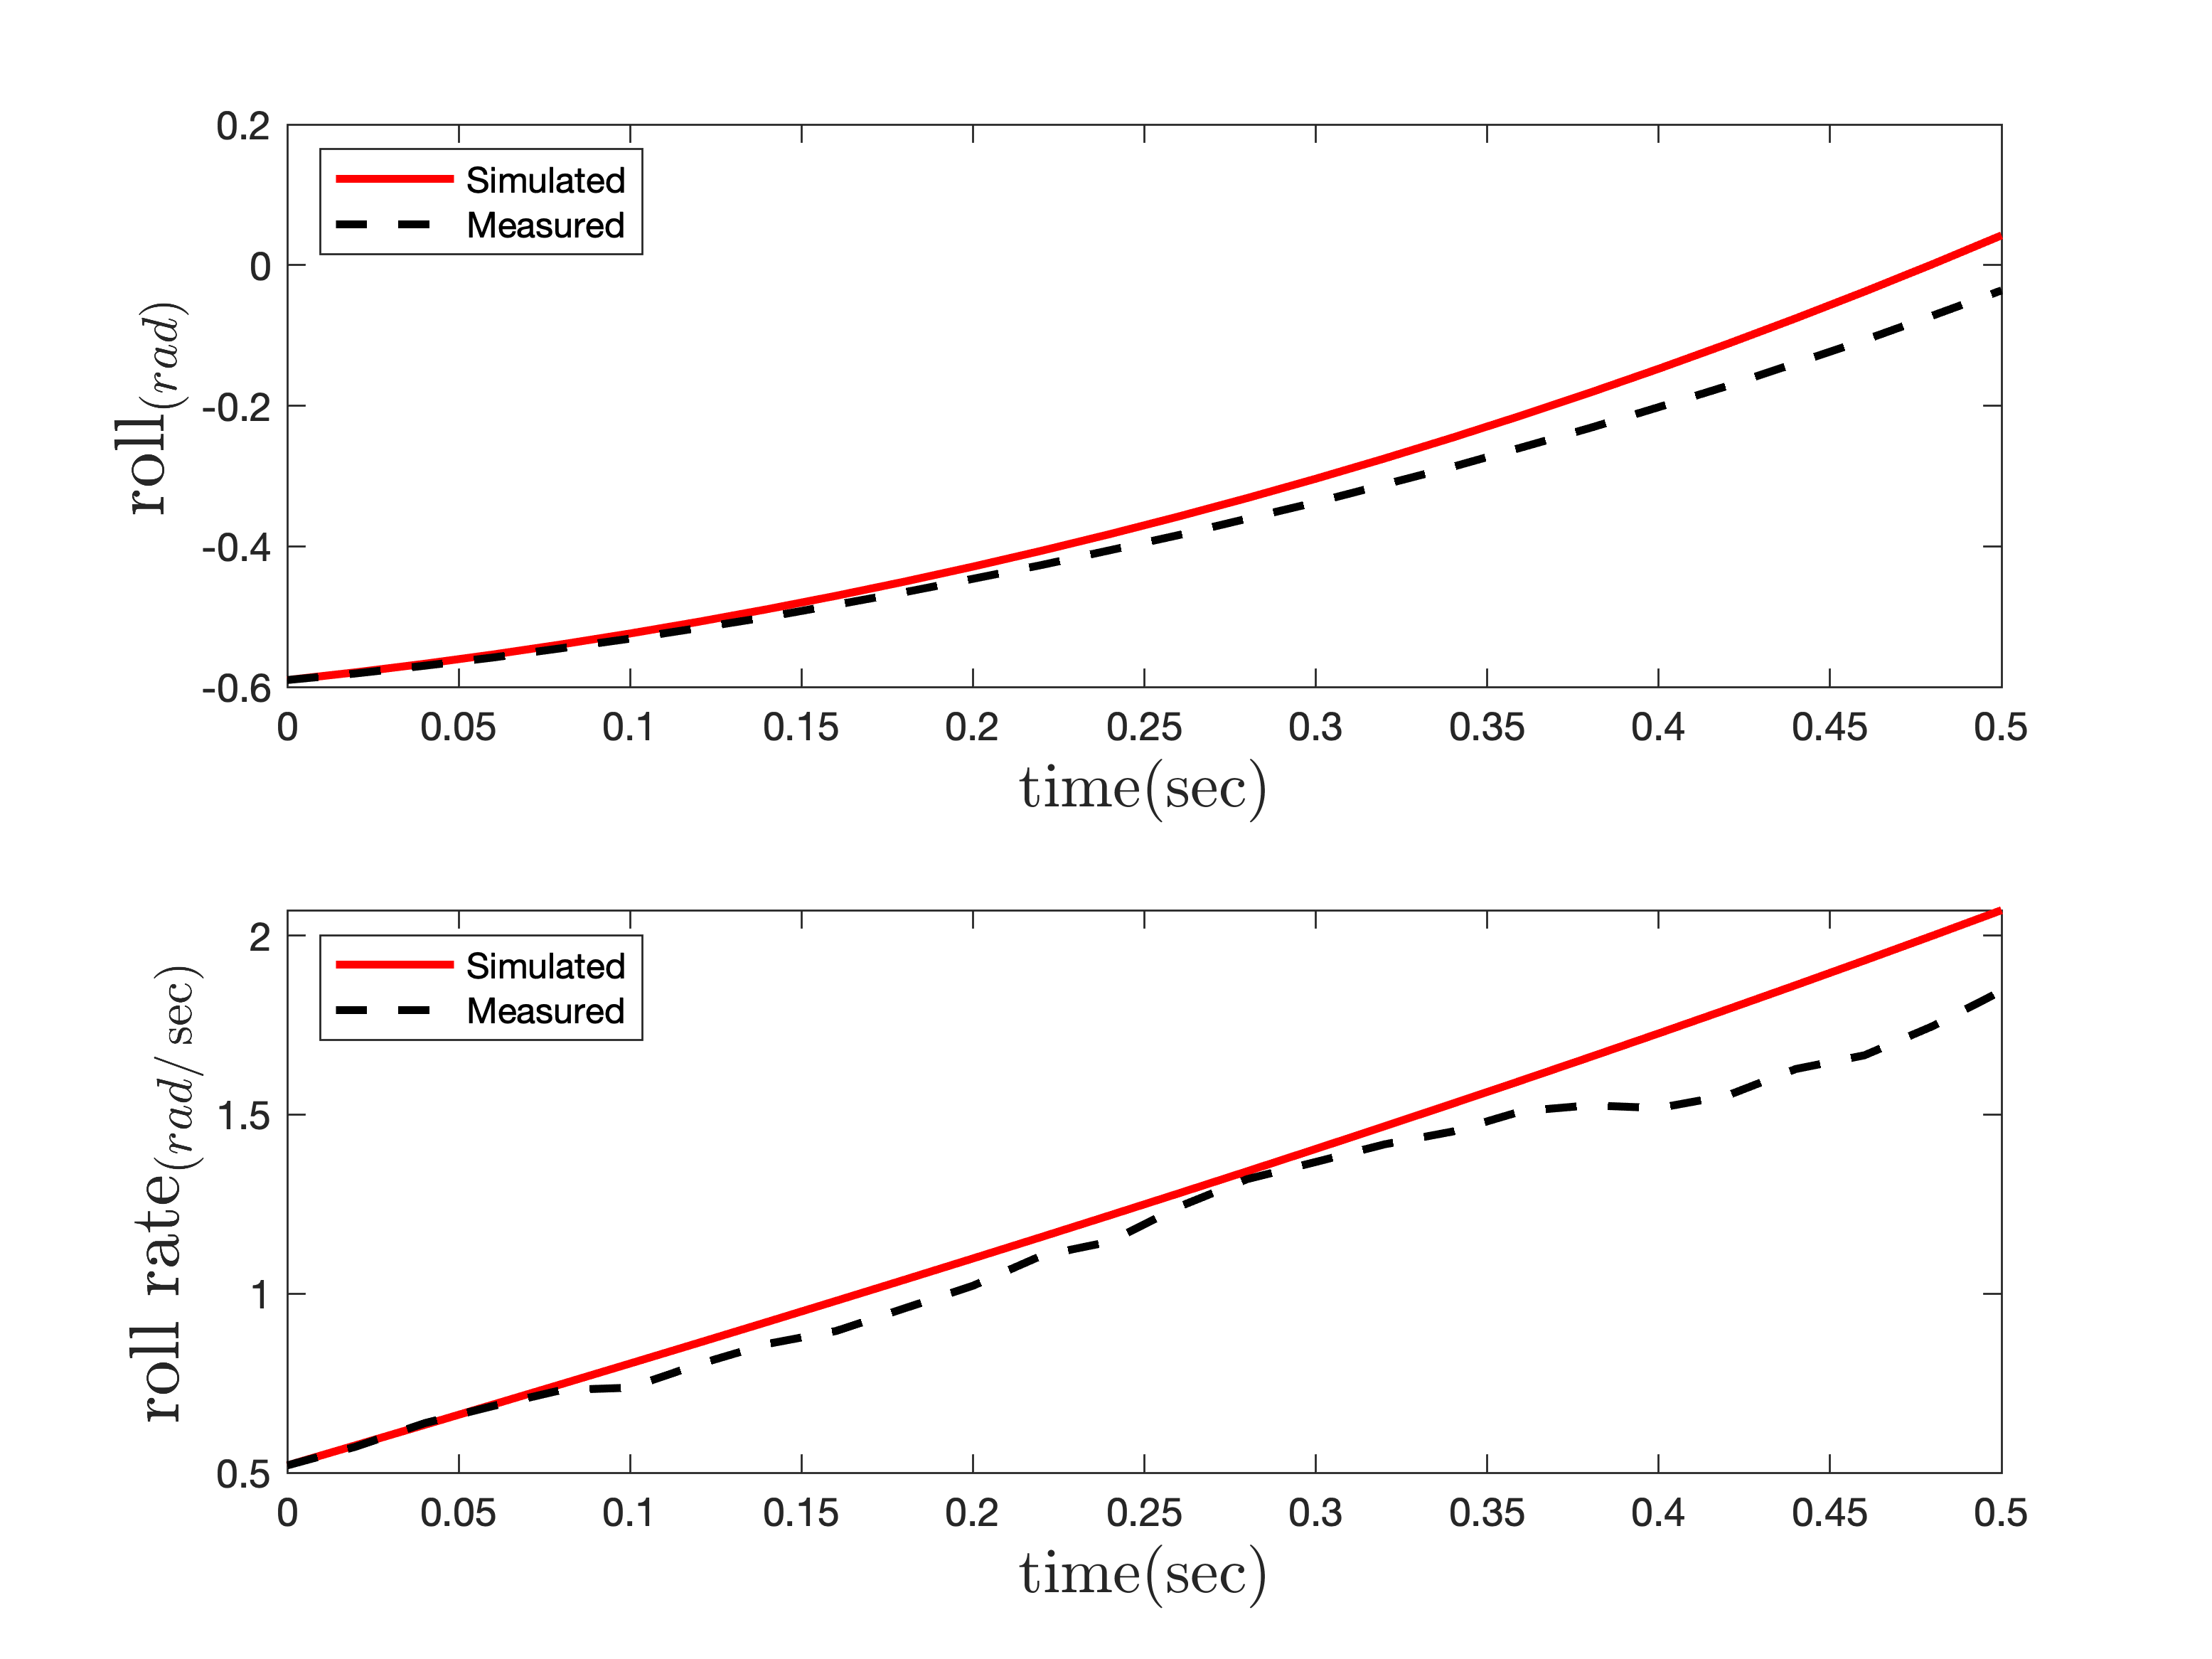
\includegraphics[width=12cm]{../Figures/RCP/roll_parameter_estimation/RCP_roll_S1.png}
%	\centering
%	\caption{مقايسه وضعیت استند در  آزمايش اول و شبیه‌سازی، پس از تخمین پارامترهای کانال رول}
%	\label{roll_ps1}
%\end{figure}
%\begin{figure}[H]
%	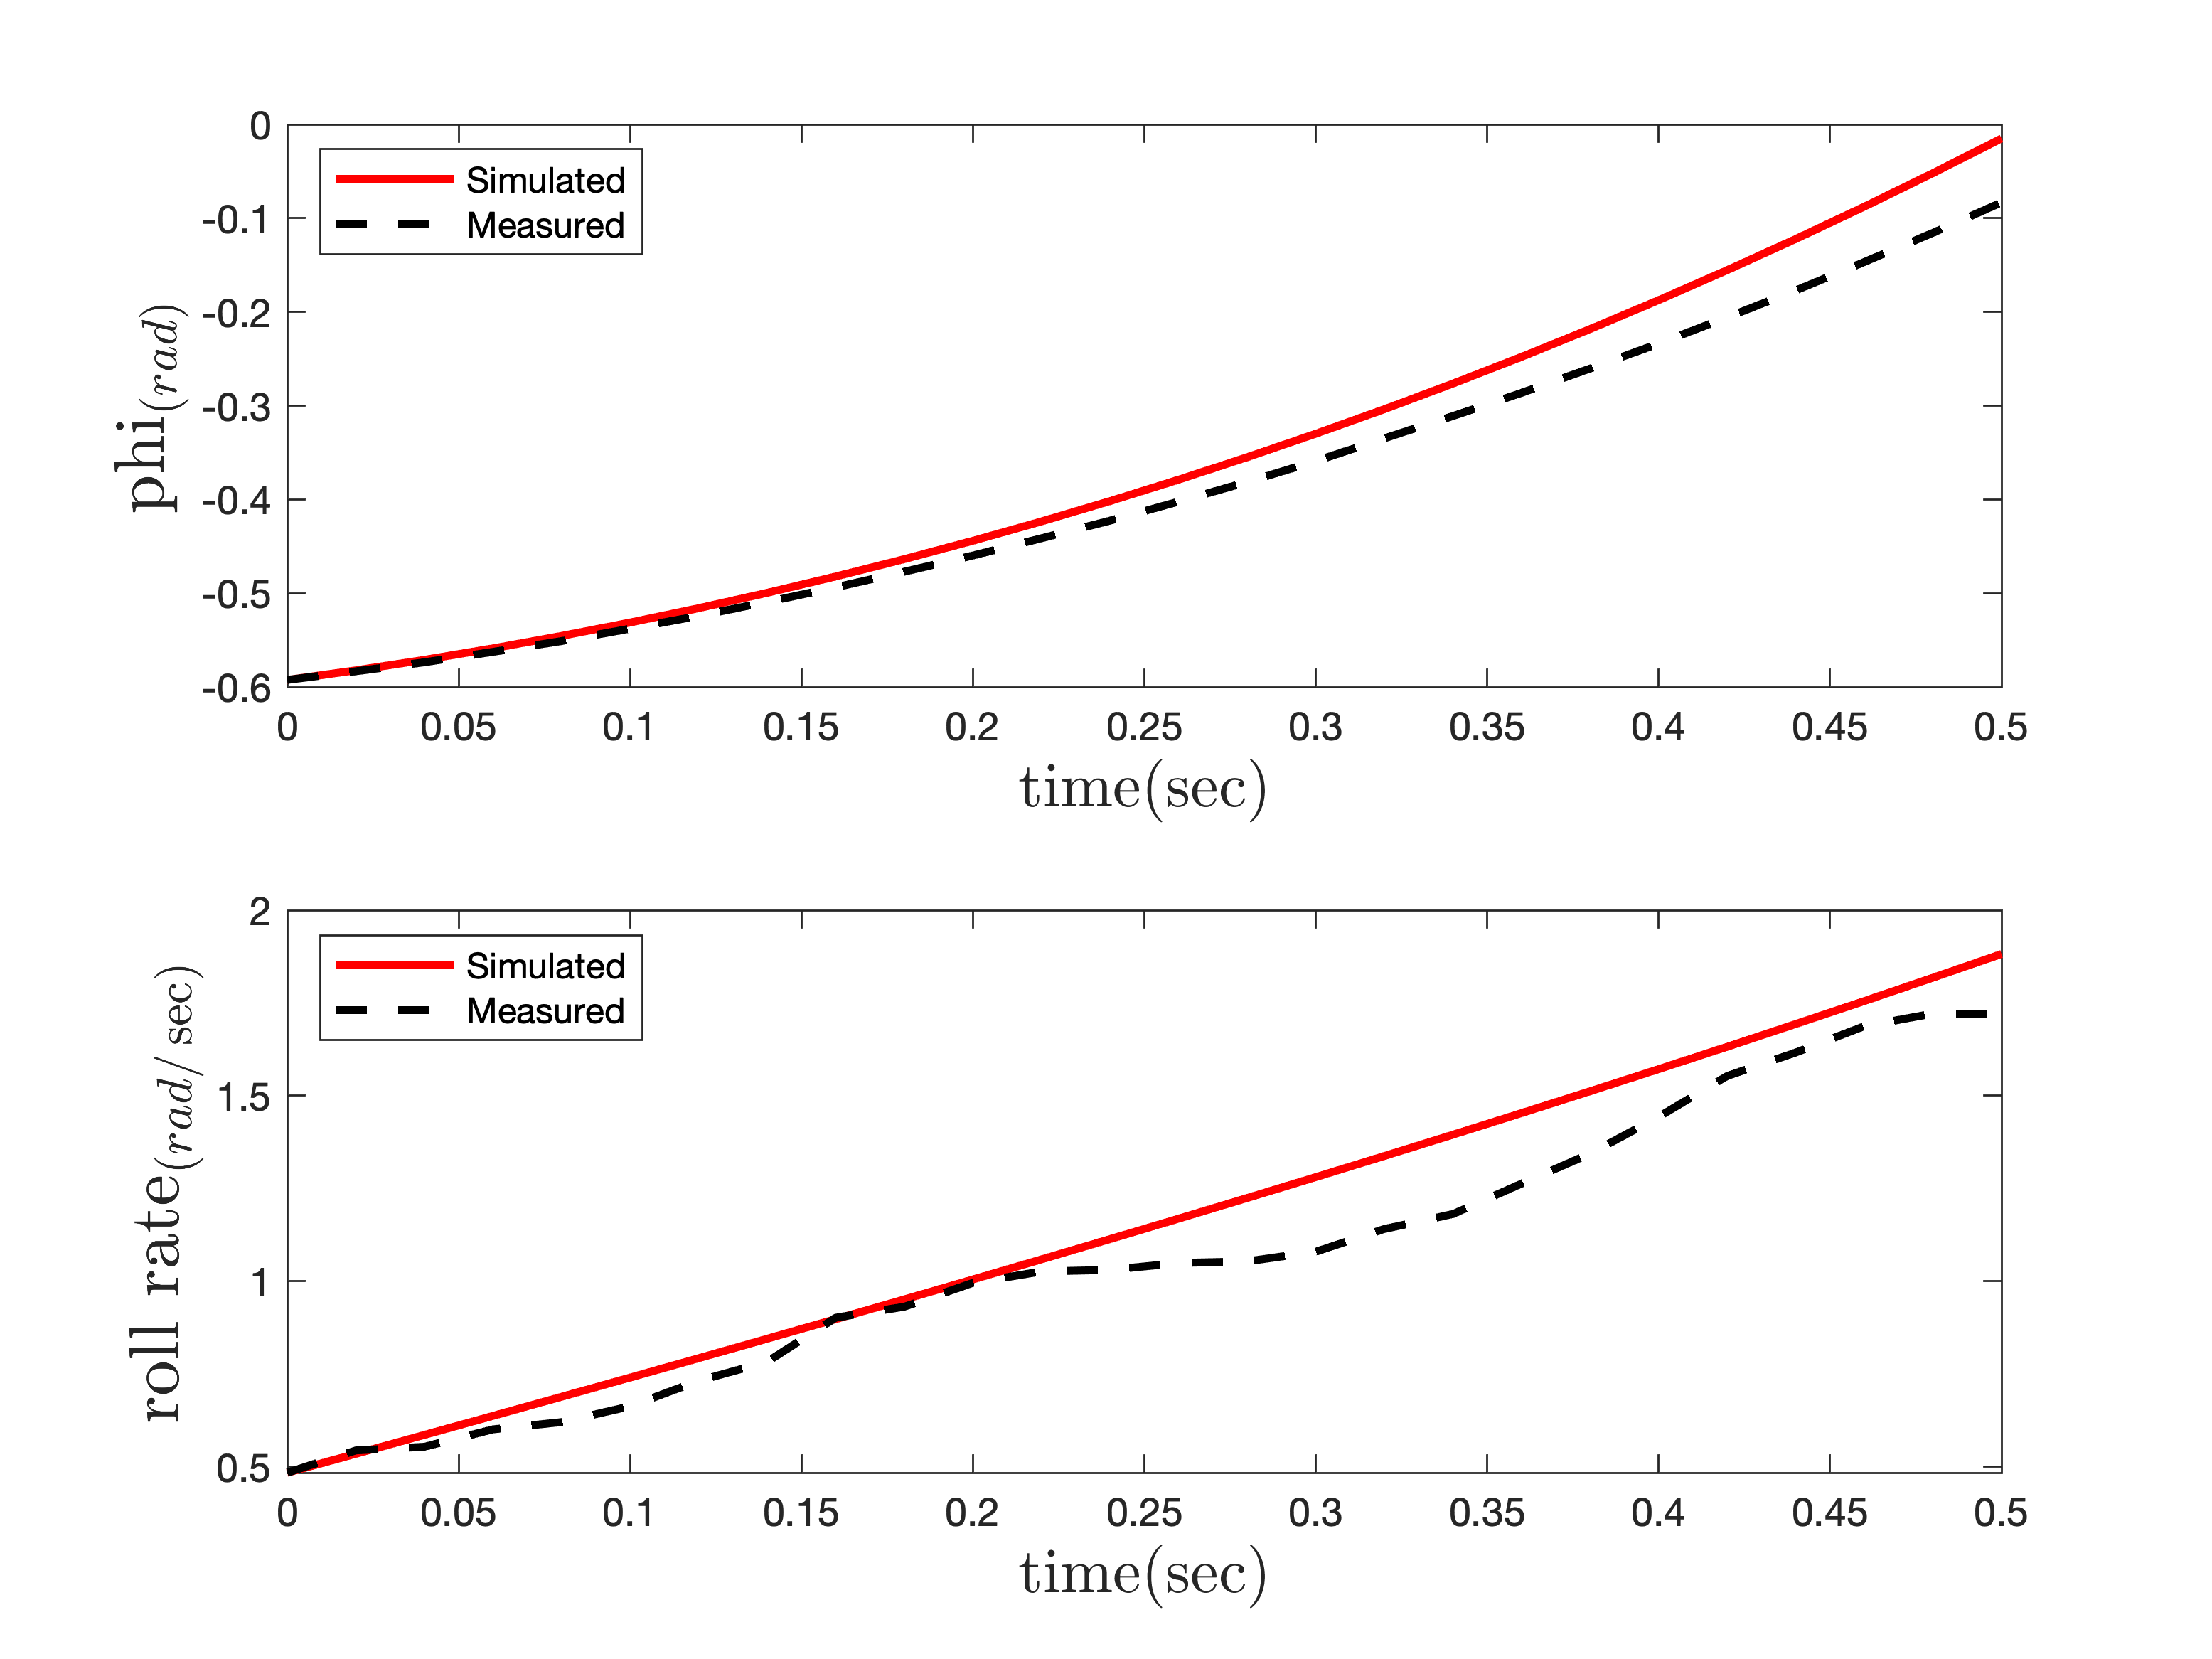
\includegraphics[width=12cm]{../Figures/RCP/roll_parameter_estimation/RCP_roll_S2.png}
%	\centering
%	\caption{مقايسه وضعیت استند در  آزمايش دوم و شبیه‌سازی، پس از تخمین پارامترهای کانال رول}
%	\label{roll_ps2}
%\end{figure}
%\begin{figure}[H]
%	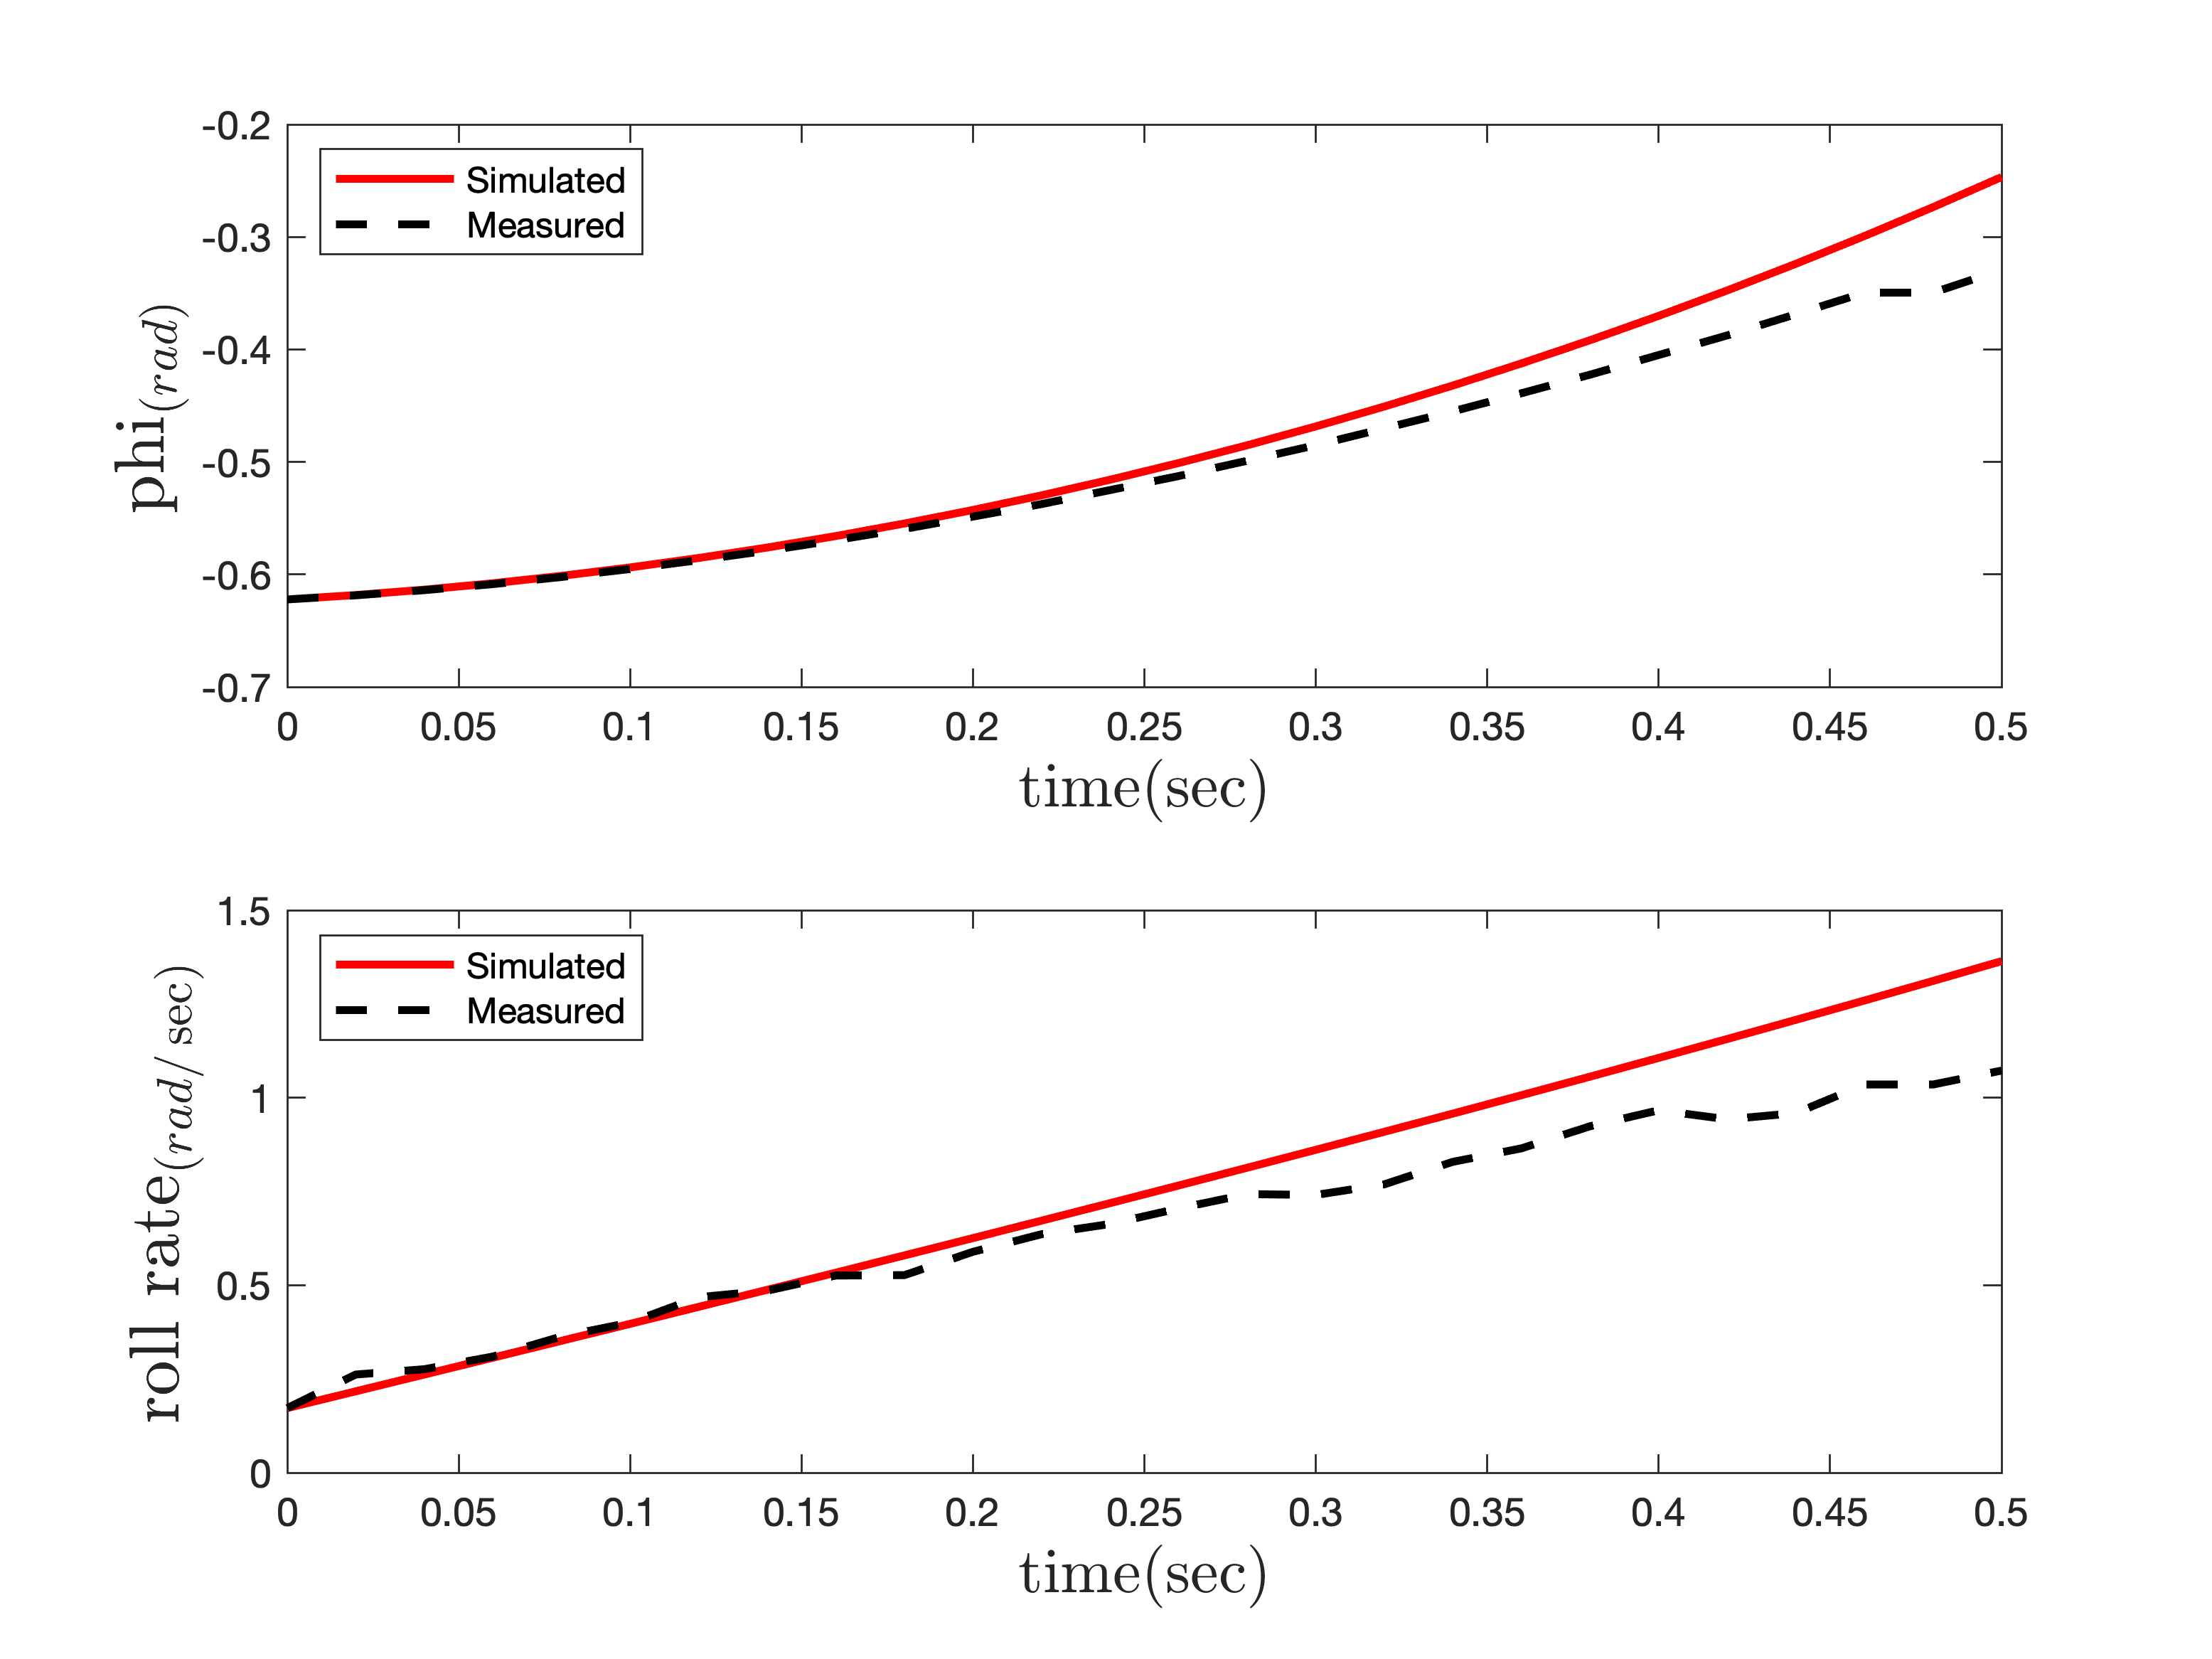
\includegraphics[width=12cm]{../Figures/RCP/roll_parameter_estimation/RCP_roll_S3.png}
%	\centering
%	\caption{مقايسه وضعیت استند در  آزمايش سوم و شبیه‌سازی، پس از تخمین پارامترهای کانال رول}
%	\label{roll_ps3}
%\end{figure}
\begin{figure}[H]
	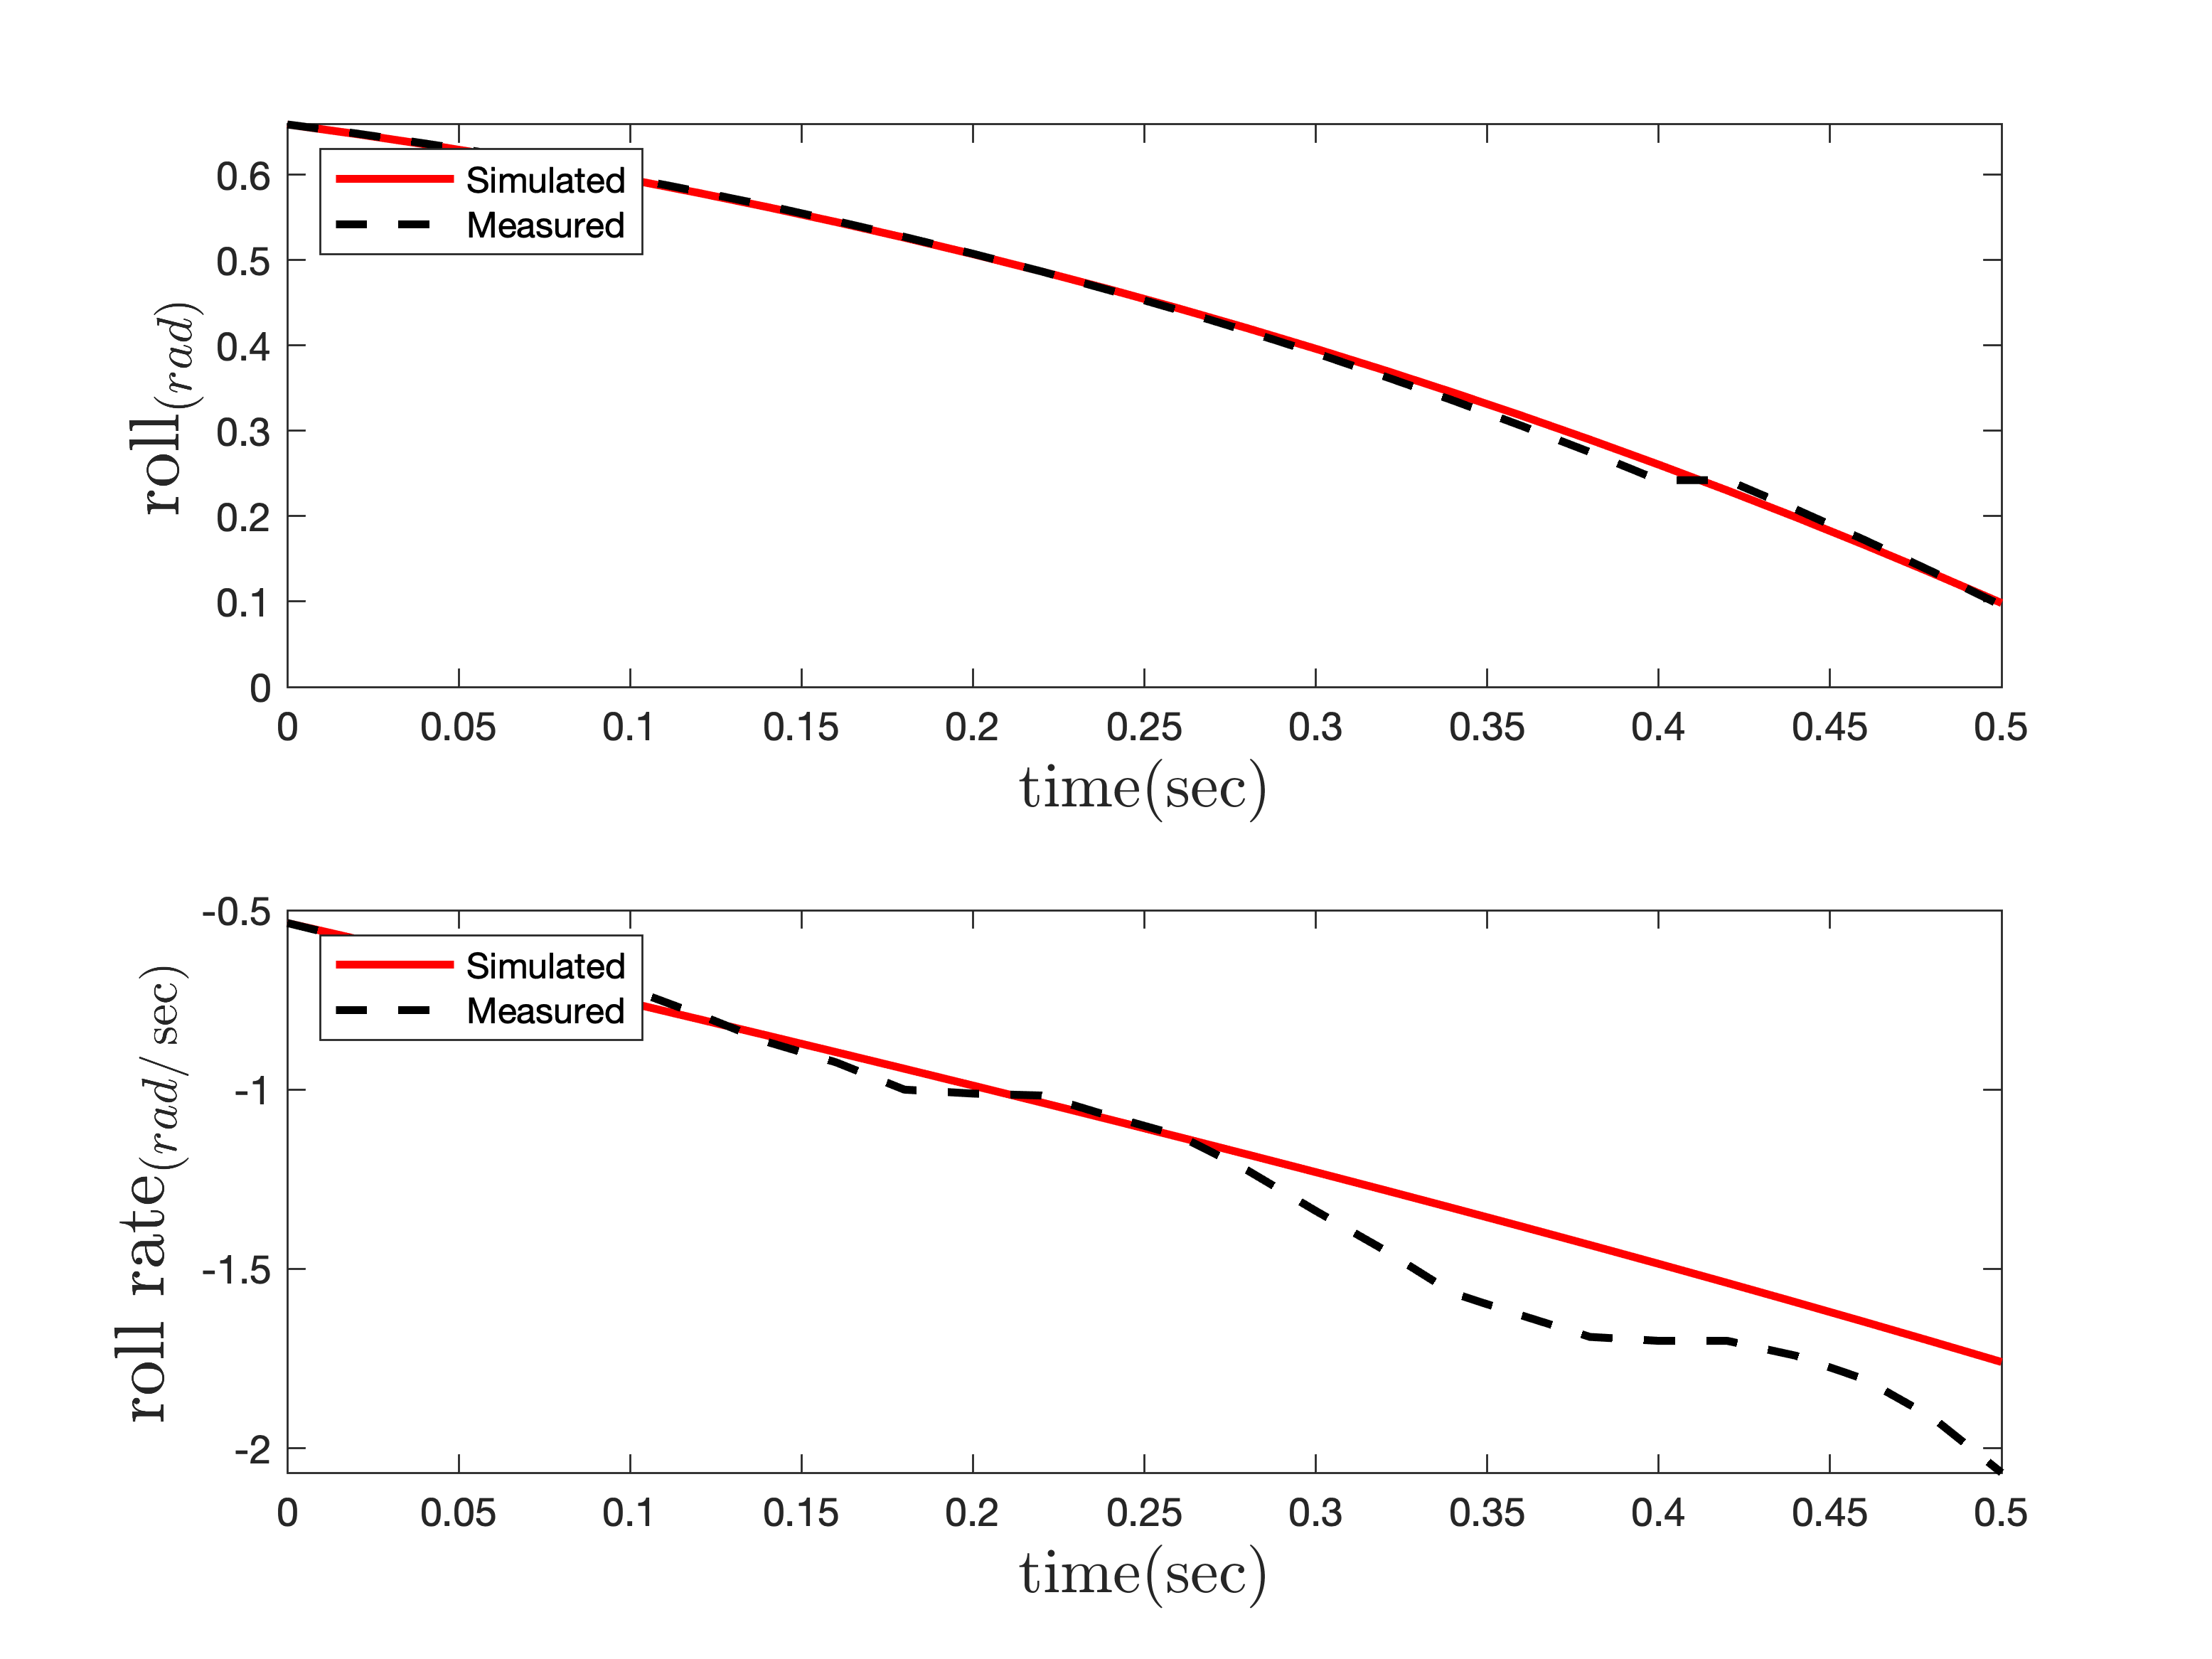
\includegraphics[width=.55\linewidth]{../Figures/RCP/roll_parameter_estimation/RCP_roll_S4.png}
	\centering
	\caption{مقايسه وضعیت استند در  آزمايش چهارم و شبیه‌سازی، پس از تخمین پارامترهای کانال رول}
	\label{roll_ps4}
\end{figure}
%\begin{figure}[H]
%	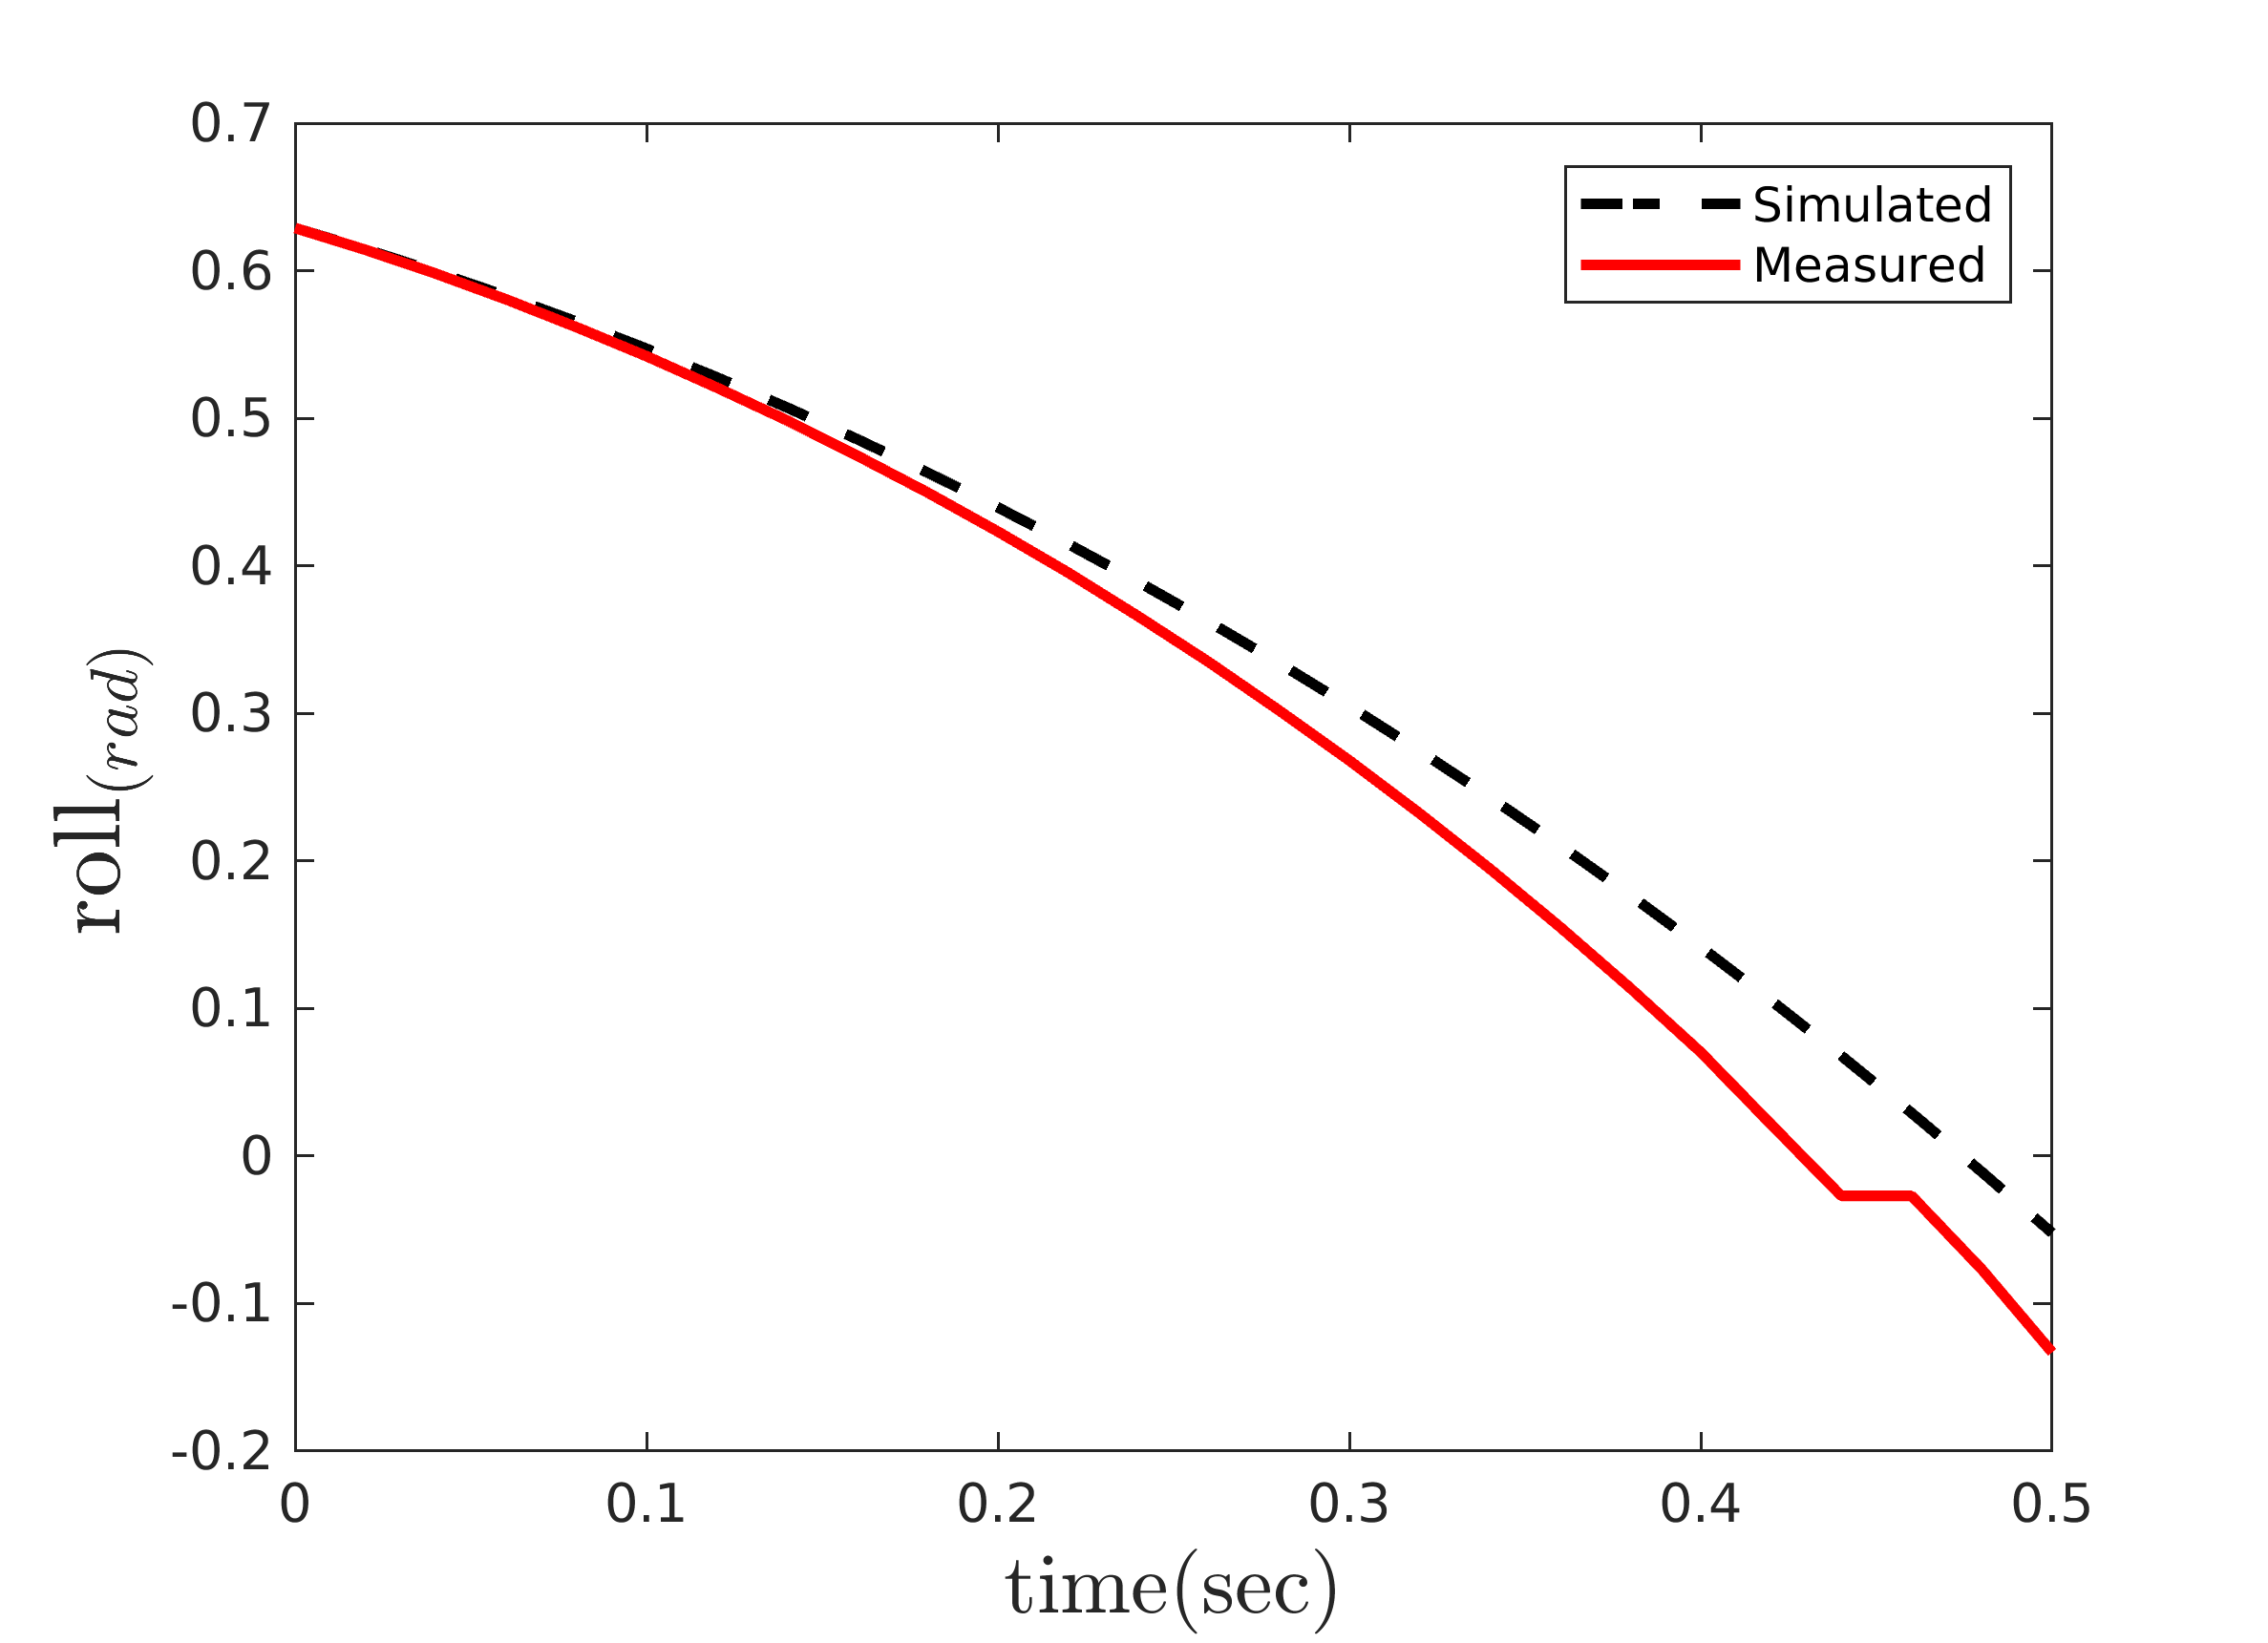
\includegraphics[width=12cm]{../Figures/RCP/roll_parameter_estimation/RCP_roll_S5.png}
%	\centering
%	\caption{مقايسه وضعیت استند در  آزمايش پنجم و شبیه‌سازی، پس از تخمین پارامترهای کانال رول}
%	\label{roll_ps5}
%\end{figure}